\subsection{Ingresos y egresos}

\subsubsection{Ingresos}
Para el plan de negocio propuesto se propone 3 planes para acceder al producto. Empezando por el plan gratuito se presenta en forma de prueba, debido a que esta dirigido a empresas interesadas en probar el producto antes de adquirirlo, los planes gold y platinum ya oficializan el interés del cliente en el negocio y se le dan beneficios de acuerdo a la membrecia que compren. En la tabla \ref{ingresos} se da una descripción mas detallada considerando el análisis mensual y anual por compañía.

\vspace{2mm}
\begin{minipage}{0.9\textwidth}
\centering
\captionof{table}[{Ingresos}]{ Ingresos. }
\label{ingresos}
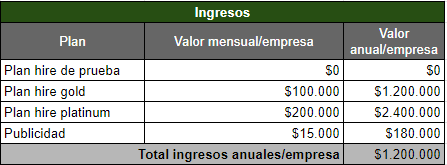
\includegraphics[width=0.7\textwidth]{Images/ingresos.png}
\fnote{Nota. \textup{Fuente : Autores}}
\end{minipage}


\subsubsection{Egresos}
En el primer año se tiene en cuenta las dos personas que lideran el proyecto y se encuentra con personal reducido que estarán pagos bajo las respectivas prestaciones y aportes parafiscales correspondientes a los recursos humanos de la empresa teniendo en cuenta la normativa Colombiana. Por otro lado se suma la infraestructura de trabajo de manera virtual. En la tabla \ref{egresos} se explica mas a detalle.

\vspace{2mm}
\begin{minipage}{0.9\textwidth}
\centering
\captionof{table}[{Egresos}]{ Egresos. }
\label{egresos}
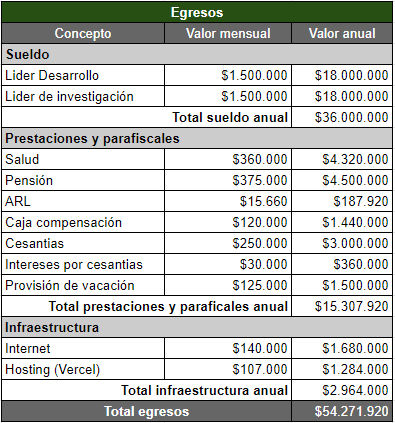
\includegraphics[width=0.7\textwidth]{Images/egresos.png}
\fnote{Nota. \textup{Fuente : Autores}}
\end{minipage}